%%%%%%%%%%%%%%%%%%%%%%%%%%%%%%%%%%%%%%%%%%%%%%%%%%%%%%%%%%%%%%%%%%%%%%%%%%%%%
\chapter{Sequence-to-Sequence Task-Oriented Dialogue Modeling}
\label{06:chap:lm-tod}
%%%%%%%%%%%%%%%%%%%%%%%%%%%%%%%%%%%%%%%%%%%%%%%%%%%%%%%%%%%%%%%%%%%%%%%%%%%%%
Task-oriented dialogue is a complex task typically modeled with architectures consisting of multiple modules \ref{02:sec:basics}.
This approach makes it challenging to transfer the learned knowledge since all the modules need to be adjusted during the transfer.

This concern can be addressed using end-to-end trainable models that can transfer the knowledge in one step and, therefore can be adjusted to different domains and use cases more easily.
In task-oriented dialogue, end-to-end implementations are dominated by sequence-to-sequence architectures based on Language Models \ref{relwork:end-to-end}.
The LM-based approaches have taken over the benchmarks \footnote{\url{https://github.com/budzianowski/multiwoz\#trophy-benchmarks}}, demonstrating SoTA performance.
However, these competitive models are fine-tuned on a single training set.
In this chapter, we raise the question of how well these models can transfer the obtained skill of leading the dialogue to other domains.
In other words, we want to discover if the models learn useful skills that can be beneficial in other domains or if the demonstrated behavior merely reproduces the patterns seen in the training portion of the data.
The work presented in this chapter was presented at the LREC conference and covered by~\citet{hudecek-etal-2022-unifying}.
For modeling, we use the AuGPT model \cite{kulhanek-etal-2021-augpt} to the development we contributed to during this work.
We also present some additional experiments regarding the smaller training set, presented in \ref{tab:exp-results-seed}

\section{AuGPT Model Description}
\label{06:augpt}
We choose the AuGPT model introduced by \citet{kulhanek-etal-2021-augpt}.
The architecture utilizes GPT-2 model~\cite{radford2019language} that is used for both belief state prediction and response generation, following the method described in Section~\ref{background:2stage-lm-modeling}.
GPT-2 is a pre-trained language model based on a Transformer decoder.
Therefore, it is suitable for modeling sequences in natural language.
AuGPT directly builds on the \emph{small} version of the model, resulting in a 124M parameter model.
Additionally, AuGPT introduces multiple training improvements.
Instead of solely using cross-entropy loss for language modeling, AuGPT uses an additional training objective for state corruption detection.
During training, the model is randomly presented with corrupted versions of the belief state.
For corruption, portions of the belief state are replaced with random values.
Several strategies can be used to create the corrupted versions; we replace the slot values randomly.
The model learns to predict if the presented belief state corresponds to the respective context in the training example.
This modification aims to improve the robustness of the belief state prediction.
Since GPT can work with any natural language sentences, it is straightforward to apply this model to our dialogue datasets.

\section{DIASER corpus introduction}
\label{06:sec:diaser}
Motivated by the questions raised in this chapter, we created a collection of several well-established task-oriented dialogue datasets spanning several domains to yield one larger multi-domain corpus.
Specifically, we used: \textbf{MultiWOZ 2.2} (MW), \textbf{Schema-guided dialogue} (SGD), \textbf{DSTC2} (DSTC) and \textbf{CamRest676} (CR).
For more details about the aforementioned datasets, please refer to Section~\ref{02:sec:input-data-desc}.

\subsection{Theoretical motivation}
Our aim is to cover as many domains as possible in a unified corpus.
Our source dataset choice is thus mainly based on the level of annotation available -- all source datasets include semantic annotation on the turn level and explicit database interaction. 
Despite the dataset similarities, important differences need to be resolved.

The main task when merging datasets is to unify the different domain-specific ontologies, i.e., the different attributes contained in the dialogue acts.
More precisely, the unified dataset ontology contains all the possible domains with corresponding slots and associated value sets.
We cannot consider the slots independently from the domain they belong to.
Indeed, a slot that represents the \textit{price range} will not have the same range of values compared to a restaurant or a flight ticket.
We identified two main problems related to this issue:
\begin{enumerate}
    \item \textbf{Name reference ambiguities}
    We need to design the final ontology so that different slot names refer to different concepts (with due precaution for label choice) and merge different slot names associated with the same value set under a single label.
    For example, in MultiWOZ, there are two different slot names \textit{day} and \textit{book-day} for the same value set (weekdays) and usage contexts.
    But in SGD, slot names may be misleading since we can find a slot named \textit{start-day} and another called \textit{day}; the former refers to a calendar date while the latter refers to a weekday.
    %In MultiWOZ again, there is a slot named \textit{leave-at} whose value is always a time frame (independently of the domain), but its dual slot called \textit{arrive-by} can be either a time frame (train domain), or a day of the week (hotel domain). \\
    %In SGD, all the following slots have exactly the same values : \{\textit{number-of-tickets,number-of-adults,people,total-people,persons,number-of-riders,group-size,number-of-seats} \}.
    
    \item \textbf{Absence of ontology/database} When the SGD dataset was collected, the authors used API calls instead of the database lookup.
    Therefore, no database-related metadata was released with the corpus, forcing us to create an ontology and a database for the data based on values occurring in the conversations.
\end{enumerate}

\subsection{Details of the merging approach}
Here, we present details on how we merged the data into a common format, including the handling of different ontologies.
Quantitative statistics of the final dataset are shown in Table~\ref{02:tab:data_stats}.
Full technical documentation can be found in the data repository.\footnote{\url{https://github.com/ufal/diaser}}
Here we list an overview of all the required merging steps:

\paragraph{Matching belief representations.} In DSTC and CR, belief state annotations are extracted from both the user and the system utterance, whereas in the MW and SGD datasets, the belief state is only extracted from the user utterance. We had to filter automatically the annotations from DSTC and CR until they matched the MW belief state representation. 
    
\paragraph{Adding meta features} from the original datasets. DSTC2, CamRest, and MultiWOZ contain the \emph{goal} of the dialogue (also called task) as a dialogue act with the constraints (e.g. expensive restaurant south) and the information the user needs to obtain from the system (e.g. phone number and address). They also contain a short text summarizing this goal for crowd workers. We include both versions of the task description with each dialogue.
    
\paragraph{Unifying annotation structure.} The final dataset structure is similar to the structure of SGD and MultiWOZ 2.2. We create a \textit{Turn} object that contains either the user utterance and dialogue acts or the system utterance.
Two consecutive entries for the user and system share the same turn number -- we consider a \textit{Turn} as an exchange between the user and the system (i.e. a pair or utterances). 

\paragraph{Ontology unification.}   
One of the most difficult parts of this work was to unify ontologies\footnote{Although none of the datasets have a formal specification or an RDF representation, the lists of all possible domains, intents, slots, and slot values are generally referred to as ontologies in dialogue systems literature, including the description papers for the source datasets.} of each original dataset because they were not built on the same dimensions.
This concerns slot, domain, and intent names. After indexing all metadata from the different datasets, we merged them manually using MultiWOZ as the pivot.
We always check the meaning in context and match slots/intents with the same semantics.

In addition to unifying the naming, we also needed to solve the following problems:
\begin{enumerate}
    \item SGD does not include any ontology information; we thus had to build the ontology from scratch based on values from the included API responses. Since SGD uses several API schemas per domain, each with its own set of slots, often using different names for the same concepts, we also unified the different schemas, the same as we did with different data sources.

    \item DSTC2 and CamRest ontologies distinguish between two kinds of slots: informable and requestable. \emph{Informable} (also called \emph{constraints}) are slots for which the value needs to be specified by the user (e.g., price, area); the user cannot specify \emph{requestable} slots but can ask the system for their value (e.g., phone number, address). We use this distinction to also assign slots in the other two datasets into one of these two groups.

\end{enumerate}

\paragraph{Slot co-reference}
Some source corpora (MW and SGD) include co-reference between slots.
For example, \textit{start-time} can take the value “sooner than that” or the slot \emph{hotel-name} can take the value “event you mentioned earlier”.
This is a problem if we assume a self-contained ontology that captures all the possible values from the corpus.


\begin{table}[tp]
    \centering\footnotesize
    \begin{tabular}{l>{\hspace{-3mm}}r>{\hspace{-2mm}}rrr>{\hspace{-2mm}}r}
        \toprule
        \bf Intent &
        \textbf{SGD} & 
        \textbf{MW} &
        \textbf{DSTC} &
        \textbf{CR} &
         \textbf{all}\\ \midrule
        \textbf{inform} & 151,467 & 84,259 & 33,451 & 5,786 & 274,963\\ 
        \textbf{request} & 81,786 & 31,888 & 13,620 & 1,516 & 128,810\\ 
        \textbf{offer} & 67,095 & 4,497 & 23,763 & 0 & 95,355\\ 
        \textbf{bye} & 35,089 & 12,380 & 0 & 0 & 47,469\\ 
        \textbf{else}& 31,030 & 13,779 & 0 & 0 & 44,809 \\ 
        \textbf{select}& 33,820 & 2,834 & 243 & 0 & 36,897\\ 
        \textbf{confirm}& 30,327 & 0 & 5,756 & 0 & 36,083\\
        \textbf{thank}& 23,172 & 9,064 & 0 & 0 & 32,326\\ 
        \textbf{negate}& 132,01 & 4,399 & 4,413 & 0 & 22,023\\ 
        \midrule
        \textbf{total}& 435,957 & 163,100 & 81,346 & 7,312 & 718,645\\
        \bottomrule
    \end{tabular}
    \caption{Most frequent intents in our unified schema, for each source and overall (with absolute numbers of occurrences).}
    \label{tab:intents}
\end{table}

\begin{table}[tp]
    \centering\footnotesize
    \begin{tabular}{l>{\hspace{-2mm}}rrrrr}
        \toprule
        \bf Slot &
        \textbf{SGD} & 
        \textbf{MW} &
        \textbf{DSTC} &
        \textbf{CR} &
         \textbf{all}\\ \midrule
        \textbf{name} & 65,999 & 42,215 & 3,135 & 2 & 111,351\\ 
        \textbf{area} & 8,133 & 48,285 & 37,697 & 4,178 & 98,293 \\ 
        \textbf{date} & 81,600 & 20,872 & 0 & 0 & 102,472\\
        \textbf{price} & 1,950 & 33,084 & 32,267 & 4,032 & 71,333\\
        \textbf{type}& 41,146 & 28,562 & 0 & 0 & 69,708\\
        \textbf{leave}& 32,625 & 26,684 & 0 & 0 & 59,309\\
        \textbf{arrive}& 26,180 & 26,228 & 0 & 0 & 52,408\\
        \textbf{food}& 13,501 & 20,963 & 3,007 & 571 & 38,042\\
        \textbf{book}& 17,618 & 11,723 & 0 & 0 & 29,341\\
        \midrule
        \textbf{total}& 298,752 & 232,388 & 76,106 & 8,783 & 532,257\\
        \bottomrule
    \end{tabular}
    \caption{Most frequent slots in our unified schema, for each source and overall (with absolute numbers of occurrences).}
    \label{tab:slots}
\end{table}

\section{Experiments}
\subsection{Exerimental setup}
For training, we follow~\citep{kulhanek-etal-2021-augpt} with the training setup
We use PyTorch framework \cite{pytorch} and run the training for 8 epochs on the MultiWOZ data when all the training examples are used.
The AuGPT model extends the \emph{small} variant of the GPT-2 model.
It consists of 12 transformer blocks with a model layer size equal to 768, having 124 million parameters in total.
For the state corruption detection task, we use a dropout of 0.1 with label smoothing of 0.1.
We use the AdamW optimizer \cite{DBLP:conf/iclr/LoshchilovH19}.
% For greater training effectiveness, we employ mixed-precision training \cite{micikevicius2017mixed} through PyTorch AMP. 
We discuss the used data in detail in Section~\ref{06:sec:diaser}
\subsection{Experiment goals}
In this chapter, we want to explore if sequence-to-sequence LM-based architectures can robustly learn the dialogue modeling capabilities and how well they can transfer them to other domains.
To answer these questions, we conduct a series of experiments to train the model using only a small portion of the training data or a completely different dataset with similar properties.

\section{Results}
We divide the results into two sections.
First, we describe the performance of the AuGPT model when trained and evaluated on various datasets.
In the second section, we show the results when the model is pre-trained on a certain dataset and then fine-tuned using only a small portion of training data from the target dataset.


\subsection{Influence of training data on the target performance}
\begin{table*}[tp]
    \centering \small
    \begin{tabular}{ccc >{\hspace{1em}} ccc >{\hspace{1em}} ccc}
      \toprule
       \multicolumn{3}{c}{training} & \multicolumn{3}{c}{evaluation} & \multicolumn{3}{c}{metrics}\\
       \textbf{DSTC} & \textbf{MW} & \textbf{SGD} & \textbf{DSTC} & \textbf{MW} & \textbf{SGD} & \textbf{Slot F1} & \textbf{JGA} & \textbf{BLEU} \\
       %========================================================
       \midrule
       %========================================================
       % mwoz-mwoz
       {\textcolor{red} \xmark} & {\textcolor{green} \cmark} & {\textcolor{red} \xmark} & {\textcolor{red} \xmark} & {\textcolor{green} \cmark} & {\textcolor{red} \xmark} & 0.89 & 0.53 & 18.61 \\
       % schema-mwoz
       {\textcolor{red} \xmark} & {\textcolor{red} \xmark} & {\textcolor{green} \cmark} & {\textcolor{red} \xmark}  & {\textcolor{green} \cmark} & {\textcolor{red} \xmark} & 0.16 & 0.02 & 4.01 \\
       % dsctmwoz-mwoz
       {\textcolor{green} \cmark} & {\textcolor{green} \cmark} & {\textcolor{red} \xmark} & {\textcolor{red} \xmark}  & {\textcolor{green} \cmark} & {\textcolor{red} \xmark} & 0.89 & {0.55} & 19.67 \\
       % dstcschema-mwoz
       {\textcolor{green} \cmark} & {\textcolor{red} \xmark} & {\textcolor{green} \cmark} & {\textcolor{red} \xmark}  & {\textcolor{green} \cmark} & {\textcolor{red} \xmark} & 0.17 & 0.03 & 5.68 \\
       % mwozschema-mwoz
       {\textcolor{red} \xmark} & {\textcolor{green} \cmark} & {\textcolor{green} \cmark} & {\textcolor{red} \xmark}  & {\textcolor{green} \cmark} & {\textcolor{red} \xmark} & 0.89 & 0.52 & 19.92 \\
       % all-mwoz
       {\textcolor{green} \cmark} & {\textcolor{green} \cmark} & {\textcolor{green} \cmark} & {\textcolor{red} \xmark}  & {\textcolor{green} \cmark} & {\textcolor{red} \xmark} &  0.90 & 0.54 & 21.09 \\
       %========================================================
       \midrule
       %========================================================
       % mwoz-schema
       {\textcolor{red} \xmark} & {\textcolor{green} \cmark} & {\textcolor{red} \xmark} & {\textcolor{red} \xmark} & {\textcolor{red} \xmark} & {\textcolor{green} \cmark} & 0.04 & 0.01 & 5.63 \\
       % schema-schema
       {\textcolor{red} \xmark} & {\textcolor{red} \xmark} & {\textcolor{green} \cmark} & {\textcolor{red} \xmark}  & {\textcolor{red} \xmark} & {\textcolor{green} \cmark} & 0.59 & 0.21 & {28.17} \\
       % dstcmwoz-schema
       {\textcolor{green} \cmark} & {\textcolor{green} \cmark} & {\textcolor{red} \xmark} & {\textcolor{red} \xmark}  & {\textcolor{red} \xmark} & {\textcolor{green} \cmark} & 0.03 & 0.01 & 5.51 \\
       % dstcschema-schema
       {\textcolor{green} \cmark} & {\textcolor{red} \xmark} & {\textcolor{green} \cmark} & {\textcolor{red} \xmark}  & {\textcolor{red} \xmark} & {\textcolor{green} \cmark} & 0.58 & 0.21 & 27.96 \\
       % mwozschema-schema
       {\textcolor{red} \xmark} & {\textcolor{green} \cmark} & {\textcolor{green} \cmark} & {\textcolor{red} \xmark}  & {\textcolor{red} \xmark} & {\textcolor{green} \cmark} & 0.63 & 0.23 & 27.54 \\
       % all-schema
       {\textcolor{green} \cmark} & {\textcolor{green} \cmark} & {\textcolor{green} \cmark} & {\textcolor{red} \xmark}  & {\textcolor{red} \xmark} & {\textcolor{green} \cmark} & 0.63 & 0.22 & 27.72 \\
       %========================================================
       \midrule
       %========================================================
       % dstcmwoz-all
       {\textcolor{green} \cmark} & {\textcolor{green} \cmark} & {\textcolor{red} \xmark} & {\textcolor{green} \cmark} & {\textcolor{green} \cmark} & {\textcolor{green} \cmark} & 0.28 & 0.12 & 15.30 \\
       % dstcschema-all
       {\textcolor{green} \cmark} & {\textcolor{red} \xmark} & {\textcolor{green} \cmark} & {\textcolor{green} \cmark} & {\textcolor{green} \cmark} & {\textcolor{green} \cmark} &  0.55 & 0.22 & 27.28 \\
       % mwozschema-all
       {\textcolor{red} \xmark} & {\textcolor{green} \cmark} & {\textcolor{green} \cmark} & {\textcolor{green} \cmark} & {\textcolor{green} \cmark} & {\textcolor{green} \cmark} & 0.65 & 0.25 & 25.13 \\
       % all-all
       {\textcolor{green} \cmark} & {\textcolor{green} \cmark} & {\textcolor{green} \cmark} & {\textcolor{green} \cmark} & {\textcolor{green} \cmark} & {\textcolor{green} \cmark} & 0.70 & 0.28 & \textbf{29.73} \\

      \bottomrule
  \end{tabular}
  \caption{Performance of the AuGPT model trained and evaluated on various subsets of the unified dataset.}
  \label{tab:exp-results-diaser}
\end{table*}

We can see a general pattern in the results suggesting that the model fails to generalize across different datasets when a subset of data we evaluate on is not included in the training. A significant drop in performance can be observed across all recorded metrics.

Regarding the $F_1$ slot score and joint goal accuracy, the explanation for the poor model's accuracy can be found in a significantly different distribution of slots across SGD/MW datasets and DSTC.
Training on MW provides us with the most reasonable scores on slot $F_1$ and joint goal accuracy.
Training on both SGD and MW brings only a very marginal improvement.
The big difference in performance can also be seen in terms of BLEU, which suggests a big difference in the language used in each dataset.

The performance of the model evaluated on MW is analogous.
Training the model solely on SGD gives us a model that cannot be generalized to MW data.
Concatenating MW datasets with SGD, DSTC, or both during training leads to a little improvement, predominantly in terms of BLEU score.
We get the best results when using the whole DIASER dataset for training and obtain the model with better generalizing capabilities supported by the BLEU score 21.09.

The model evaluation on SGD data mostly follows the same pattern. However, in this case, it is quite interesting to observe that training the model on the whole DIASER is not beneficial, and the performance stagnates, although the training set is much bigger.

Finally, if we evaluate the whole DIASER dataset, it is clear that the best-performing model is obtained when we train it on the full data.
Table \ref{tab:exp-results-diaser} shows that including SGD data is crucial for achieving higher BLEU values while training on MW helps the model predict slot values.

\subsection{Dynamics of Successful and Failed Dialogues}
We also perform a detailed quantitative analysis of errors made by the trained models.
To do so, we evaluated the AuGPT model trained on the MW data regarding the dialogue success rates.
We only chose the MW data due to additional annotation in MultiWOZ.
We consider dialogue success as defined in Section~\ref{02:sec:eval_metrics}
``All failed" corresponds to applying this model to our dialogue datasets is straightforward, while ``all success" corresponds to dialogues for which both conditions were met and, therefore, were successful.
It is thus an evaluation concerning the dialogue as a whole, unlike the turn-level methods, such as evaluating the system's response generation.

In Figure~\ref{fig:error_distr}, we provide a histogram of errors in successful and failed dialogues.
We go turn by turn and identify the errors in the dialogue state predicted by the system compared to the expected state.
In particular, we show the count of cases where some information is understood wrongly by the system (positive values) or is missing completely (negative values).
We can see that in successful dialogues, the system might make some mistakes at first but can recover eventually.
On the other hand, most dialogue failures are caused by missing information in the second half of the dialogue, which suggests that the recovery is not certain.

We further identify four reasons that can cause an error:
\begin{enumerate}
    \item \emph{Domain} is wrongly identified.
    \item \emph{Intent} is detected wrongly.
    \item Some \emph{inform} value is captured incorrectly.
    \item Some \emph{request} was not answered.
\end{enumerate}
We realized some observations:
\begin{itemize}
    \item For both successful and unsuccessful dialogues, the first turn concentrates the most errors.
    
    \item Generally speaking, the failed dialogues show much superfluous information in the first five speech turns, especially regarding the user's intent. On the other hand, from approximately the fourth speech turn onwards, there is a lot of missing information, especially at the level of the dialogue domain. If we add the missing information with the superfluous information, the error distribution peaks between turns three and seven of the dialogue. 
    
    \item It is interesting to note that we have a significant amount of superfluous information for the first four turns in successful dialogues.
    It matches the period in which the entropy grows the most, which interestingly connects the entropy analysis and the model behavior. We hypothesize that there is a correlation between mistakes made by the system and the entropy amount variation.
\end{itemize}

\begin{figure}[tp]
    \centering  \small
    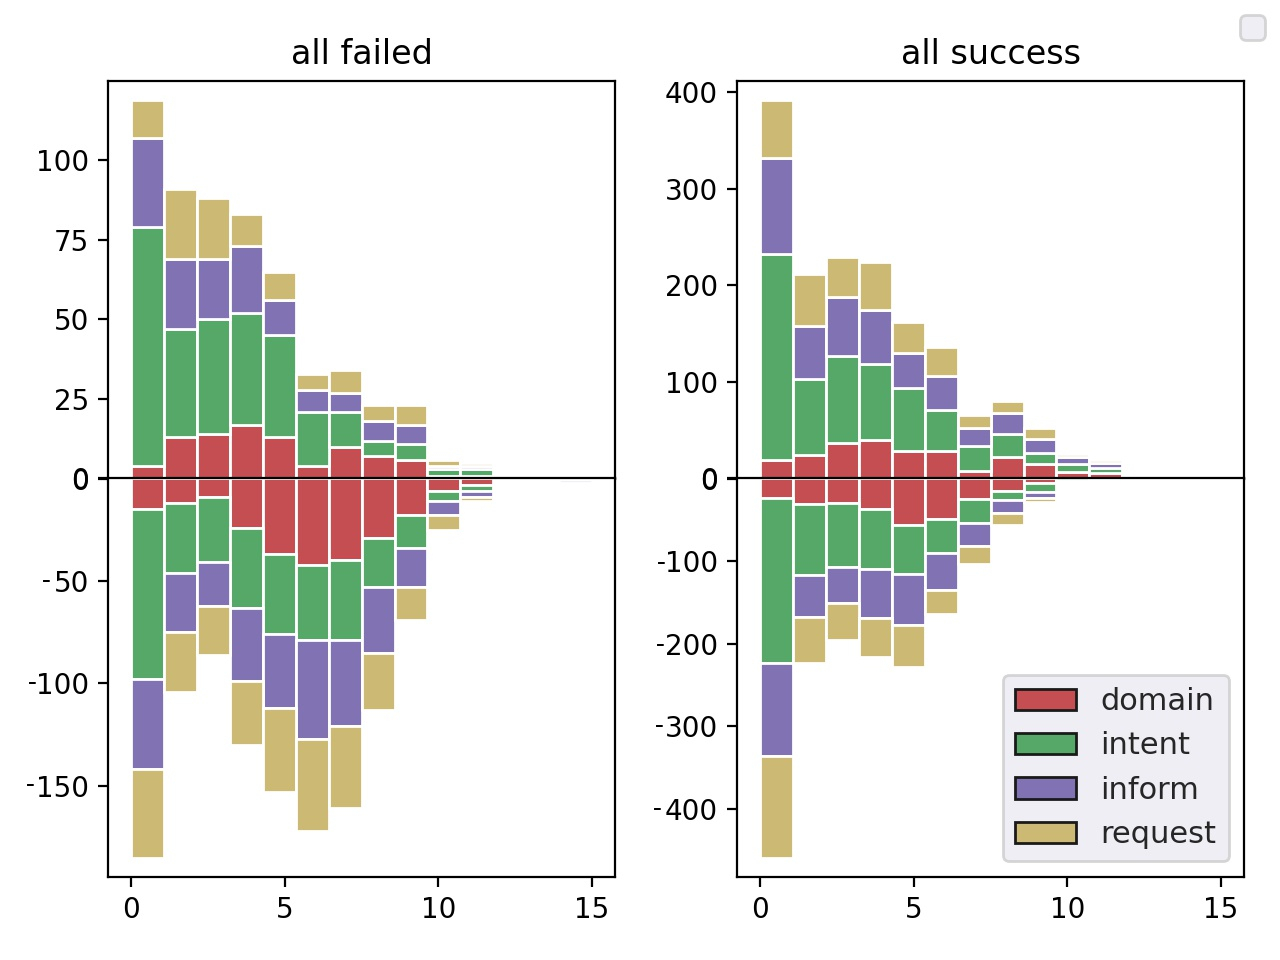
\includegraphics[width=0.49\textwidth]{images/hist-vert-True-gpt.jpg}
    \caption{Distribution and types of dialogue failures that occurred with the GPT2-based model on the MultiWOZ data.
    The horizontal axis corresponds to turn numbers. Positive values represent cases where the information is captured wrongly, while negative values represent cases where particular information is missing.
    The source of error (bad domain or intent, missing information, or not providing a request) is depicted using colors.}
    \label{fig:error_distr}
\end{figure}


\subsection{Domain adaptation with small in-domain set}
In~\ref{tab:exp-results-seed}, we present results for domain adaptation experiments.
We first train the AuGPT model on the MultiWOZ dataset and then use a small portion of the SGD data to adapt the model to this different dataset.
The results show, that although pertaining on MultiWOZ helps slightly to improve the final BLEU score, the performance of belief state tracking is not significantly improved and the results are overall rather inconclusive.

\begin{table*}[tp]
    \centering \small
    \begin{tabular}{cccccc}
      \toprule
       pre-training & fine-tuning & ft-ratio & \textbf{Slot-F1} & \textbf{JGA} & \textbf{BLEU} \\
        \midrule
       -- & SGD & 100\% & 0.59 & 0.21 & 28.17 \\
       -- & SGD & 10\% & 0.47 & 0.15 & 20.13 \\
       MW & SGD & 10\% & 0.46 & 0.16 & 19.46 \\
       -- & SGD & 5\% & 0.29 & 0.08 & 14.65 \\
       MW & SGD & 5\% & 0.29 & 0.12 & 15.16 \\
       -- & SGD & 1\% & 0.07 & 0.03 & 6.37\\
       MW & SGD & 1\% & 0.06 & 0.01 & 8.40 \\
       -- & SGD & 0.5\% & 0.04 & 0.04 & 3.43 \\
       MW & SGD & 0.5\% & 0.04 & 0.02 & 5.95 \\
       %========================================================
       \midrule
       %=======================================================
      \bottomrule
  \end{tabular}
  \caption{Performance of the AuGPT model trained and evaluated on various subsets of the unified dataset.}
  \label{tab:exp-results-seed}
\end{table*}

\section{Conclusion}
In this work, we unified a large task-oriented dialogue corpora at both data and annotation levels, which requires a complex process of merging ontologies. 
We showed that additional data from other sources helps train LM-based end-to-end dialogue models when converted to the unified format.
Although the new dataset is still far from perfect coverage, it is a step towards wider and more authentic data.
We also performed experiments to explore the ability of LM-based systems to adapt to new domains easily with a small number of in-domain examples.
The results were inconclusive, and they suggest that using in-domain data for domain adaptation is not straightforward.